\documentclass[10pt]{beamer}

\usetheme{Montpellier}
\usecolortheme{whale}

\usepackage[T1]{fontenc}
\usepackage{lmodern}

\usepackage{mathtools}
\usepackage[binary-units]{siunitx}
\usepackage{amsmath}
\usepackage{listings}
\usepackage{mdframed}
\usepackage{adjustbox}
\usepackage{minted}
\usepackage{xcolor}

\usepackage{parskip}
\usepackage{substr}
\usepackage{hyperref}
\usepackage{etoolbox}
\usepackage{tipa}
\usepackage{cprotect}
\usepackage{booktabs}
\usepackage{silence}
\usepackage[backend=biber, style=ieee]{biblatex}
\usepackage[english,ngerman]{babel}
\usepackage{csquotes}

\definecolor{lg}{gray}{0.95}
\hypersetup{colorlinks = true, urlcolor=blue, linkcolor=white}
\WarningFilter{biblatex}{Patching footnotes failed}

\renewcommand*{\bibfont}{\tiny}
\renewcommand{\subsectionname}{AA}

\bibliography{resources.bib}

\title{\textbf{Operating Systems}}
\subtitle{Tutorial 7}
\author{Fabian Klopfer}
\date{\today}

\defbeamertemplate{subsection page}{mine}[1][]{%
  \begin{centering}
    {\usebeamerfont{subsection name}\usebeamercolor[fg]{subsection name}#1}
    \vskip1em\par
    \begin{beamercolorbox}[sep=12pt,center]{part title}
      \usebeamerfont{subsection title}\insertsubsection\par
    \end{beamercolorbox}
  \end{centering}
}

\defbeamertemplate{section page}{mine}[1][]{%
  \begin{centering}
    {\usebeamerfont{section name}\usebeamercolor[fg]{section name}#1}
    \vskip1em\par
    \begin{beamercolorbox}[sep=12pt,center]{part title}
      \usebeamerfont{section title}\insertsection\par
    \end{beamercolorbox}
  \end{centering}
}

\setbeamertemplate{section page}[mine]
\setbeamertemplate{subsection page}[mine]

\begin{document}
\frame{\titlepage}


\begin{frame}{Intro}
\begin{itemize}
 \item Pingo Polls
 \item This time: extended pointer treatment
 \item Starting next time: Loaders 
\end{itemize}
\end{frame}

\section*{Exercise Sheet 6}
\frame{\sectionpage}
\subsection*{Exercise 1}
\frame{\subsectionpage}
\begin{frame}[allowframebreaks, fragile]{Exercise 1}
    \begin{enumerate}
		\item Does the difficulty of a software implementation of the Least-Recently-Used algorithm lie in converting virtual addresses to physical addresses or in handling page faults? Explain your answer. \\
		\alert{
		\begin{itemize}
		 \item Address translation: needs to be fast, that's why it's usualy impl. in HW. 
		 \item Alter field of page table on each address translation
		 \item How to make it so fast with SW?
		 \item Page faults: Occur less often, allowed to be slower
		\end{itemize}
		}
		
		\item Name two paging algorithms that can be considered approximations of the Least-Recently-Used algorithm. \\
		\alert{Not frequently used, not recently used}
		
		\framebreak
		\item Name two key challenges in implementing paging systems.\\
		\alert{Speed \& Size: \\
		\begin{itemize}
		 \item Speed as address translation happens often 
		 \item Size as address spaces are large but the page table should be small in-memory
		\end{itemize}
		}
		
		\item What property must a process have in terms of its memory accesses for a translation lookaside buffer to increase the speed of memory accesses?\\
		\alert{It has to make a large number of references to a small number of pages. \textbf{Locality} of access}
		\framebreak
		
		\item Name three advantages of virtualizing operating systems.\\
		\alert{
		\begin{itemize}
		 \item Simpler Maintenance
		 \item Simpler Migration
		 \item Simpler Testing
		 \item Less prone to crashes of the whole system/isolation
		\end{itemize}

		}
		
		\item What is a ``world switch''?\\
		\alert{Transition between hypervisor and guest}
		\framebreak
		
		\item Name two differences between virtualization and containers. \\
		\alert{Virtualization: Virtualizes HW, isolates OSes \\
		Containers: Virtualize OSes, isolate processes}
		
		\item For what reason can a hardware-based approach to virtualization (CPU support) be slower than a binary translation-based software approach? \\
		\alert{Many traps when using HW-based virtualization}
	\end{enumerate}
\end{frame}

\subsection*{Exercise 2}
\frame{\subsectionpage}
\begin{frame}[allowframebreaks, fragile]{Exercise 2}
    	\begin{enumerate}
		\item A machine instruction that loads a 32-bit word from memory into a register on the CPU can cause up to four page faults. How? \\ \vspace{0.3cm}
		\alert{Operation is on boundary $\Rightarrow 2$ page faults \\
                both operands may be on boundary $\Rightarrow 2$ page fault for each}
		\item%
			48-bit addresses, \SI{8}{\kibi\byte} sized pages.
			How many pages does a single-level linear page table contain? \\ \vspace{0.3cm}
			\alert{ $\frac{2^{48}}{8\cdot1024} = 2^{48} / 2^{13} = 2^{35} = 34,359,738,368 \approx$ 34 million.}
			\framebreak
		\item%
			virtual address space \SI{64}{\kibi\byte}, page size \SI{4}{\kibi\byte}.
			A process has \SI{32768}{\byte} program code, \SI{16386}{\byte} data and \SI{15870}{\byte} stack.
			Does the process fit into the address space? \\ \vspace{0.5cm}
			\alert{System has $64 / 4 = 16$ pages.\\
			Code, data and stack have each \\
			$\SI{32768}{\byte} = 8 \cdot \SI{4096}{\byte} + \SI{0}{\byte}$, \\
			$\SI{16386}{\byte} = 4 \cdot \SI{4096}{\byte} + \SI{2}{\byte}$, \\
			$\SI{15870}{\byte} = 3 \cdot \SI{4096}{\byte} + \SI{3582}{\byte}$ \\
			Thus $8 + 5 + 4 = 17$ pages \\
			Process does \textbf{not} fit into the address space.
			}
			\framebreak
		\item%
			Now page size \SI{512}{\byte}.
			Does the process now fit into the address space? \\ \vspace{0.5cm}
			\alert{System has $65,536 / 512 = 128$ pages.\\
			Code, data and stack have each \\
			$\SI{32768}{\byte} = 64 \cdot \SI{512}{\byte} + \SI{0}{\byte}$, \\
			$\SI{16386}{\byte} = 32 \cdot \SI{512}{\byte} + \SI{2}{\byte}$, \\
			$\SI{15870}{\byte} = 30 \cdot \SI{512}{\byte} + \SI{510}{\byte}$ \\
			Thus $64 + 33 + 31 = 128$ pages \\
			Process does fit into the address space.
			}
	\end{enumerate}
\end{frame}

\subsection*{Exercise 3}
\frame{\subsectionpage}
\begin{frame}[allowframebreaks, fragile]{Exercise 3}
Which page is evicted when using the following strategies?
	\begin{minipage}[t]{0.5\linewidth}
	 \vspace{1cm}
		\begin{tabular}[t]{@{}ccccc@{}}
			\toprule
			      & Load & Last & \\
			Page &  time & Access & R & M \\
			\midrule
			0 & 170 & 437 & 0 & 0 \\
			1 & 335 & 436 & 0 & 1 \\
			2 & 65 & 512 & 1 & 1 \\
			3 & 99 & 501 & 1 & 0 \\
			\bottomrule
		\end{tabular}
	\end{minipage}%
	\begin{minipage}[t]{0.45\linewidth}		
		\medskip

		\begin{enumerate}
			\item First-In First-Out \\ \alert{$\min{\text{load time}} = 65$ \\ $\Rightarrow \text{Page } 2$}
			\item Second Chance \\ \alert{$\min{\text{load time}} |_{R = 0} = 170$ \\ $\Rightarrow \text{Page } 0$}
			\item Least-Recently-Used \\ \alert{$\min{\text{last access}} = 436$ \\ $\Rightarrow \text{Page } 1$}
			\item Not-Recently-Used \\ \alert{$\text{random} |_{R = 0 \wedge M = 0}$ \\ $\Rightarrow \text{Page } 0$}
		\end{enumerate}

	\end{minipage}
\end{frame}

\subsection*{Exercise 4}
\frame{\subsectionpage}
\begin{frame}[allowframebreaks,fragile]{Pointers Again}
 \begin{itemize}
  \item Pointer $\equiv$ Variable storing an address
  \item \mintinline{c}{*} Operator returns the value at the address stored by the variable/pointer
  \item \mintinline{c}{&} Operator returns the address of the variable itself
 \end{itemize}
 \framebreak
 
     \begin{figure}
        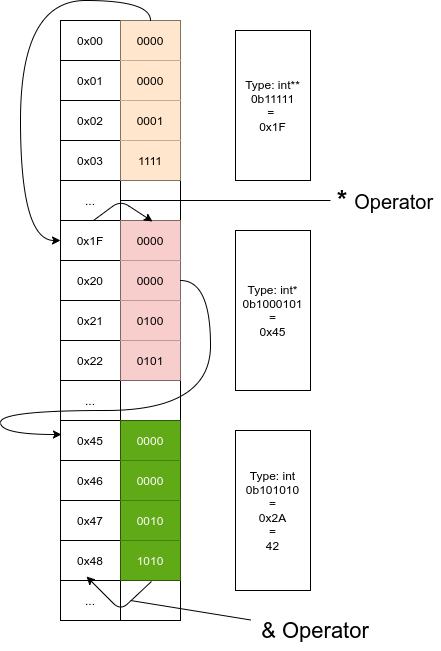
\includegraphics[keepaspectratio, width=\textwidth, height=\textheight-2\baselineskip-2\baselineskip]{img/double_ptr.png} \\
    \end{figure}
    \framebreak
 
 \adjustbox{varwidth=\textwidth, scale=0.7}{\inputminted{c}{code/test.c}}
 \framebreak
 
    \begin{figure}
        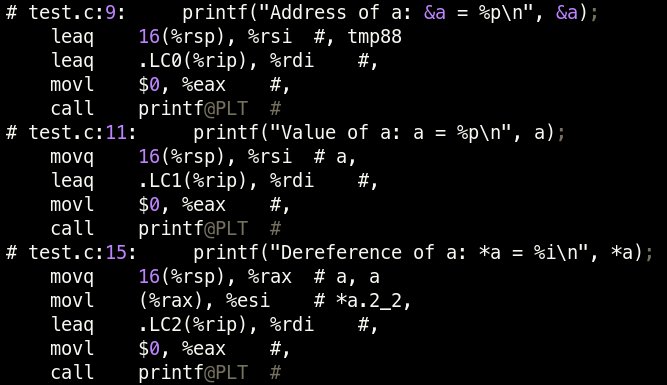
\includegraphics[keepaspectratio, width=\textwidth, height=\textheight-2\baselineskip-2\baselineskip]{img/ptr_asm.png} \\
    \end{figure}
    \framebreak
 
    \begin{figure}
        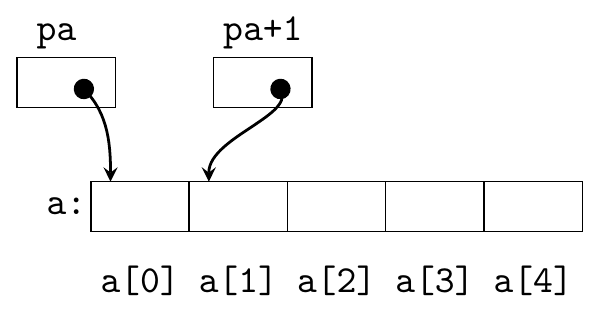
\includegraphics[keepaspectratio, width=\textwidth, height=\textheight-2\baselineskip-2\baselineskip]{img/array_ptr.png} \\
    \end{figure}
    \framebreak
    
    \begin{figure}
        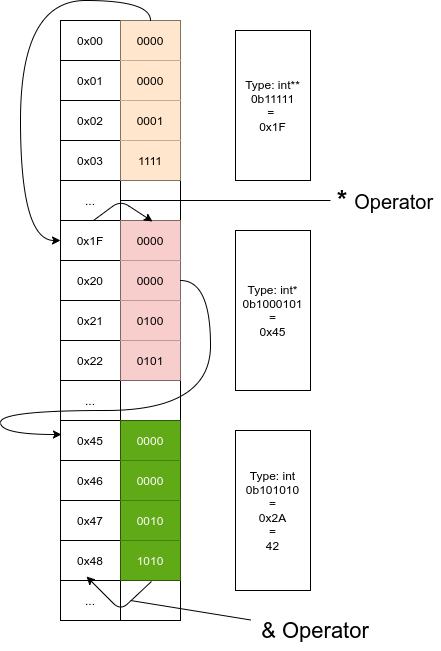
\includegraphics[keepaspectratio, width=\textwidth, height=\textheight-2\baselineskip-2\baselineskip]{img/double_ptr.png} \\
    \end{figure}
    \framebreak
    
    \begin{figure}
        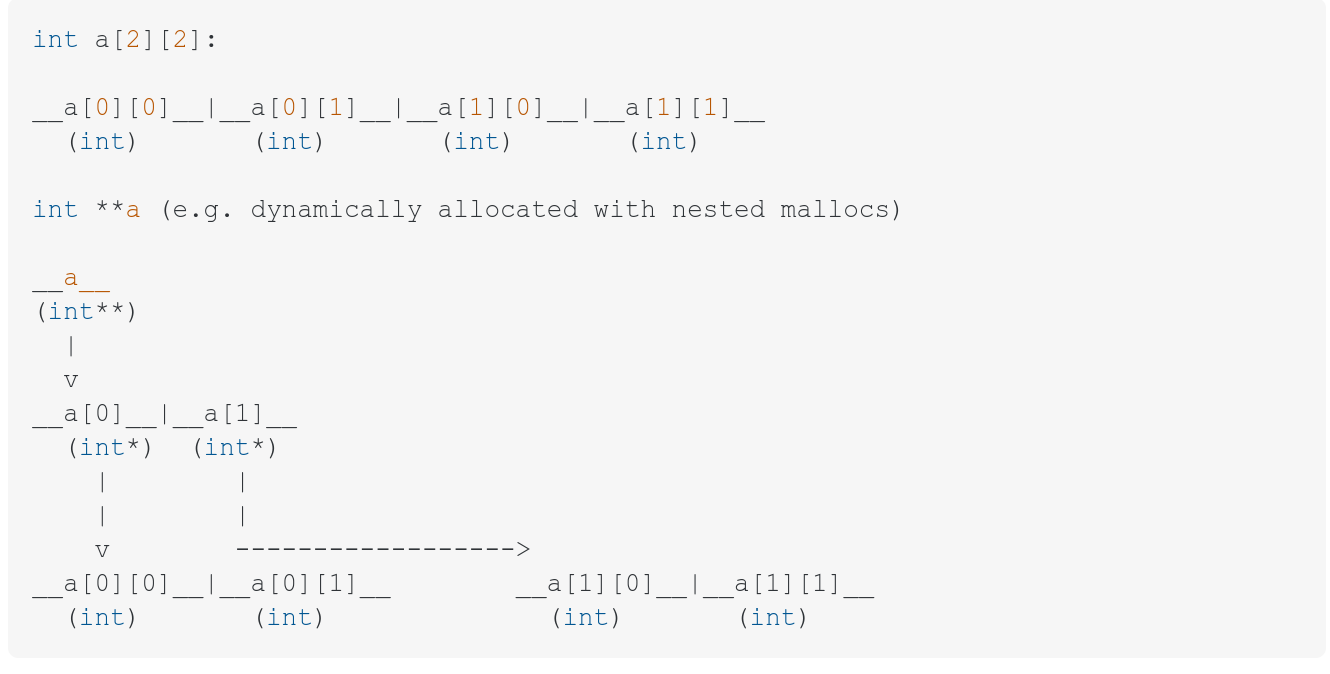
\includegraphics[keepaspectratio, width=\textwidth, height=\textheight-2\baselineskip-2\baselineskip]{img/double_ptr_mem.png} \\
    \end{figure}
    \framebreak
    Double pointers and 2D arrays and pointer to arrays example
\end{frame}

\begin{frame}[allowframebreaks, fragile]{Exercise 4}
    What output does this program produce?
	Explain your answer.

	\begin{minted}[autogobble]{c}
        #include <stdio.h>
        
        int main(void)
        {
            int a[3][2] = {{1, 2}, {3, 4}, {5, 6}};
            
            /* 1 */ printf("%d\n", a[0][0]);
            /* 2 */ printf("%d\n", **a);
            /* 3 */ printf("%d\n", *(*a + 1));
            /* 4 */ printf("%d\n", **(a + 1));
            /* 5 */ printf("%d\n", **(&a[0] + 1));
            /* 6 */ printf("%d\n", *( ((int *)(a + 2)) - 1 ));
            
            return 0;
        }
	\end{minted}
	    \begin{enumerate}
        \item 1, Prints the first value of the first subarray
        \item 1, prints the starting address of the array which is also the staring address of the first subarray which is the first element of the first subarray
        \item 2, adds one integer step to the address of the first element of the first subarray
        \item 3, adds one step to the address of the outer array, i.e. gets the address of the first element of the second subarray
        \item as above
        \item the innermost addition adds two subarray steps to the address of the array, i.e. this is the address of the third subarray. by subtracting one, we arrive at the second element of the second subarray, i.e. 4 is printed
    \end{enumerate}
\end{frame}

\subsection*{Exercise 5}
\frame{\subsectionpage}
\begin{frame}[allowframebreaks, fragile]{Exercise 5}
	Let $s$ denote the average process size in bytes, 
	let $p$ denote the size of a page in bytes, 
	and let $e$ denote the size of a page table entry in bytes.
	
	\begin{enumerate}
		\item%
			Construct an expression (in $p,s,e$) for the average memory consumption (per process) for paging (single-level page table).
		\item%
			Interpret your expression in terms of page size~$p$.
		\item%
			Determine the optimal page size~$p$ in your model.
        \framebreak
        
    \begin{figure}
        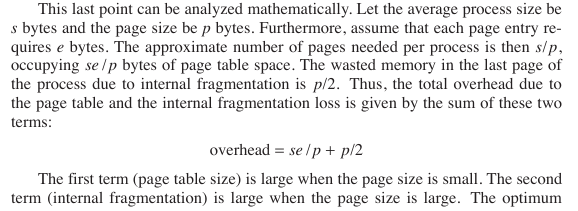
\includegraphics[keepaspectratio, width=\textwidth, height=\textheight-2\baselineskip-2\baselineskip]{img/ex5_tanen.png} \\
    \end{figure}
     \begin{figure}
        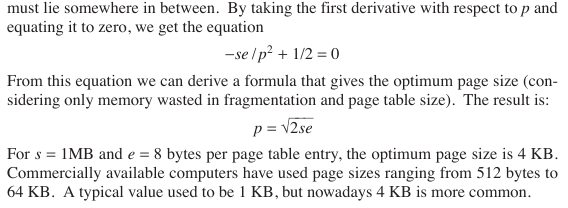
\includegraphics[keepaspectratio, width=\textwidth, height=\textheight-2\baselineskip-2\baselineskip]{img/ex5_tanen_1.png} \\
    \end{figure}   
    \framebreak
		\item%
			Calculate the optimal page size~$p$ according to your model for 
			(a) $s = \SI{1}{\mebi\byte}, e = \SI{8}{\byte}$ \\
			\alert{$p = \SI{4}{\kibi\byte}$} \\ 
			(b) $s = \SI{16}{\gibi\byte}, e = \SI{32}{\byte}$. \\
			\alert{$p = \SI{1}{\mebi\byte}$}
	\end{enumerate}
\end{frame}

    
\section*{Exercise sheet 7}
\frame{\sectionpage}
\begin{frame}[allowframebreaks, fragile]{}
 \begin{figure}
           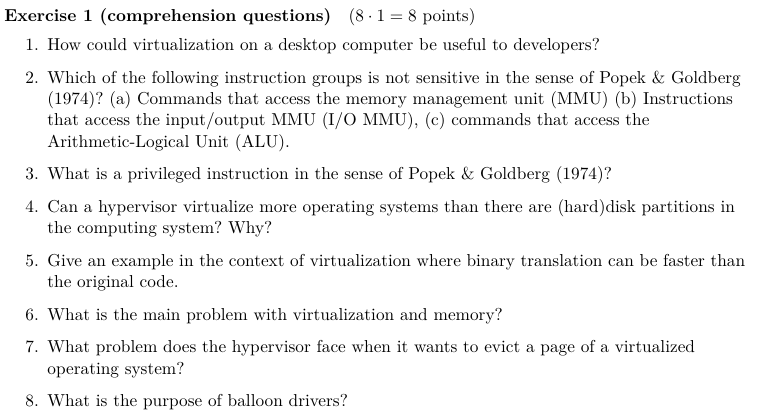
\includegraphics[keepaspectratio, width=\textwidth, height=\textheight-2\baselineskip-2\baselineskip]{img/ex6_100.png} \\
        \end{figure}
        \begin{itemize}
         \item All in the book, virtualization (chapter 7)
        \end{itemize}
        \framebreak
        
  \begin{figure}
          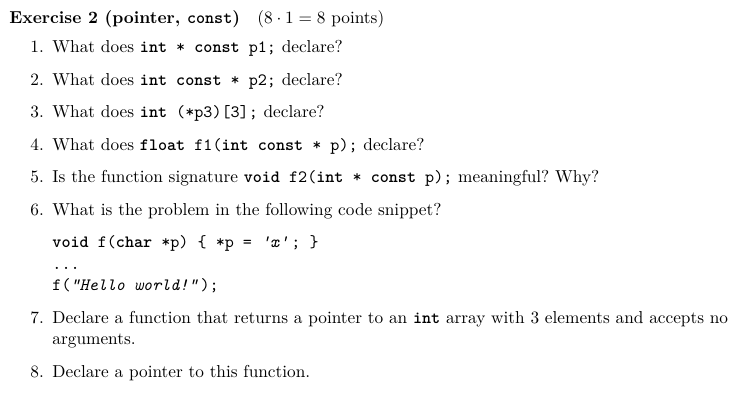
\includegraphics[keepaspectratio, width=\textwidth, height=\textheight-2\baselineskip-2\baselineskip]{img/ex6_101.png} \\
        \end{figure}
        \begin{itemize}
         \item const binds to the next symbol to the right of the type to its left
         \item \mintinline{c}{char * const a} is of "`type"' pointer and constant 
         \item address the pointer stores may not be changed.
         \item How about \mintinline{c}{char const *a}? 
         \item Of type char and \mintinline{c}{*a} cannot be changed \\
         \item Careful with const!
         \end{itemize}
        \framebreak
        
         \begin{figure}
          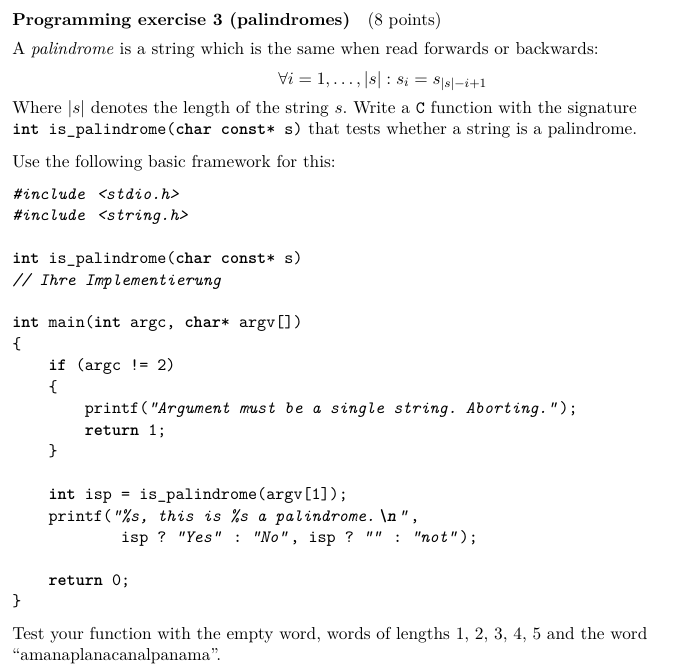
\includegraphics[keepaspectratio, width=0.8\textwidth, height=0.8\textheight-2\baselineskip-2\baselineskip]{img/ex6_102.png} \\
        \end{figure}
        \begin{itemize}
         \item Start with the string reverse code
         \item add a condition in the loop to compare the characters from front and back
        \end{itemize}
        \framebreak 
        
         \begin{figure}
          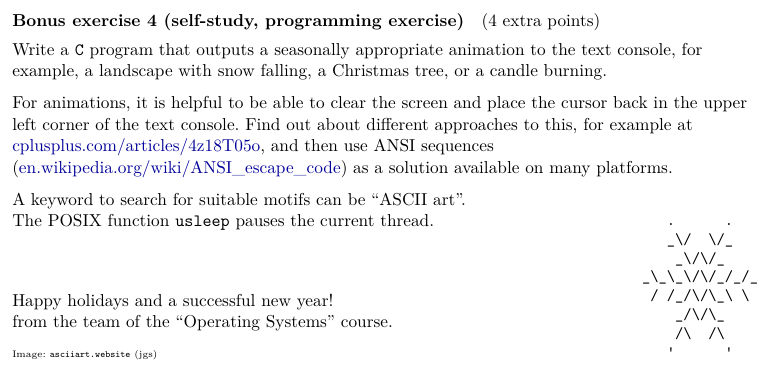
\includegraphics[keepaspectratio, width=\textwidth, height=\textheight]{img/ex6_103.png} \\
        \end{figure}
\end{frame}

\section{References}
    \begin{frame}[allowframebreaks]
      \frametitle{References}
      \begin{tiny}
      \nocite{*}
      \printbibliography
      \end{tiny}
    \end{frame}


\end{document}
 
